\chapter{Implementierung}
Die Umsetzung der zu Beginn genannten Funktionalitäten wird innerhalb der folgenden Teilabschnitte beschrieben. Der erste Teilabschnitt dieses Kapitels dokumentiert die entwickelte Software \cite{badps2}, welche den Mikrocontroller steuert und den Programmablauf der einzelnen Funktionalitäten zeigt. Der zweite Teil dieses Kapitels erläutert den Aufbau der Elektronik und zeigt wie die verwendete Hardware mit dem Mikrocontroller zusammengebaut wurde.



\section{Softwaredokumentation}
Die implementierten Softwarekomponenten \cite{badps2} gliedern sich in die drei Abschnitte für die jeweiligen Funktionalitäten, die Aufnahme von Tastatureingaben, die Wiedergabe von Tastatureingaben mittels SD-Karte und die Wiedergabe von Tastatureingaben über Ethernet. Diese beinhalten Hilfsfunktionen für die Tastatur, für die SD-Karte und für die Webseite, welche vorab in den nächsten Abschnitten beschrieben werden. Abschließend wird der gesamte Programmablauf beschrieben, der aus den Standardfunktionen des Arduino Mikrocontroller besteht und den Wechsel zwischen den Funktionalitäten ermöglicht.

\subsection{Hilfsfunktionen für die Tastatur}
\subsubsection{void initKeys(int dataPin, int clockPin)}
\subsubsection{void setHigh(int pin)}
\subsubsection{void setLow(int pin)}
\subsubsection{unsigned char readKeys(int dataPin, int clockPin)}
\subsubsection{void sendKeys(int dataPin, int clockPin, unsigned char data)}
\subsubsection{void writeKeys(unsigned char data)}


\subsection{Hilfsfunktionen für die SD-Karte}
Die implementierten Hilfsfunktionen für die SD-Karte werden benötigt, um sowohl die mitgelesenen Tastatureingaben abzuspeichern, als auch abgespeicherte Tastatureingaben wiederzugeben. Hierfür werden bestehende Funktionen aus der SD-Bibliothek von Arduino verwendet \cite{arduino_sd}. Zu beachten ist, dass Dateinamen nicht als String, sondern nur als Char-Array anzugeben sind.

\subsubsection{void initCard(int sdPin)}
Mit dieser Methode wird eine Verwendung einer SD-Karte ermöglicht, weshalb sie aufgerufen werden muss bevor eine der folgenden Hilfsfunktionen für die SD-Karte verwendet wird. Zuerst Dann wird gerprüft, ob die SD-Karte überhaupt vorhanden ist.

\subsubsection{String readFile(char* filename)}
Die Methode nimmt den Dateinamen einer Datei als Parameter entgegen und gibt einen String zurück, welcher den Textinhalt der Datei darstellt. Zunächst prüft die Methode, ob die Datei mit dem Namen existiert. Im Fall dass diese existiert, wird die Datei mit Leserechten geöffnet und solange sie verfügbar ist wird der Inhalt Zeichen für Zeichen ausgelesen und zu einem String zusammengefügt. Anschließend wird die Datei geschlossen und dieser String zurückgegeben. Falls die Datei nicht verfügbar ist, wird eine entsprechende Fehlermeldung auf der Konsole zurückgegeben.

\subsubsection{void writeFile(char* filename, String content)}
Mithilfe dieser Methode ist es möglich Daten in Form eines Strings in eine bestimmte Datei zu schreiben. Hierfür werden sowohl der Dateiname als auch der String dieser Funktion als Parameter übergeben. Die Datei mit dem übergebenen Namen wird mit Schreibrechten geöffnet und falls die Datei noch nicht existiert, wird sie automatisch erstellt. Anschließend wird überprüft, ob die Datei erfolgreich geöffnet werden konnte. Im Erfolgsfall wird der String an den bisherigen Inhalt der Datei angehangen und die Datei danach geschlossen. Andernfalls wird eine entsprechende Fehlermeldung auf der Konsole zurückgegeben.

\subsubsection{void deleteFile(char* filename)}
Diese Methode nimmt einen Dateinamen als Parameter entgegen und führt einen Löschungsbefehl für eine Datei mit diesem Dateinamen auf der SD-Karte aus. Anschließend wird geprüft, ob eine Datei mit dem Dateinamen noch existiert. Falls dies nicht der Fall ist, wird eine Nachricht ausgegeben, dass die Datei erfolgreich gelöscht wurde. Andernfalls wird eine Fehlermeldung ausgegeben.


\subsection{Hilfsfunktionen für die Webseite}
\subsubsection{void sendWebsite(EthernetClient client, String serverState)}


\subsection{Aufnahme von Tastatureingaben}
\begin{figure}
  \centering
  %\includegraphics[angle=90,width=1\textwidth]{images/diagram_reader.png}
  \caption{Aktivitätsdiagramm für die Methode reader()}
  \label{diagram_reader}
\end{figure}


\subsection{Wiedergabe von Tastatureingaben mittels SD-Karte}
\begin{figure}
  \centering
  %\includegraphics[angle=90,width=1\textwidth]{images/diagram_writer.png}
  \caption{Aktivitätsdiagramm für die Methode writer()}
  \label{diagram_writer}
\end{figure}


\subsection{Wiedergabe von Tastatureingaben über Ethernet}
\begin{figure}
  \centering
  %\includegraphics[angle=90,width=1\textwidth]{images/diagram_sender.png}
  \caption{Aktivitätsdiagramm für die Methode sender()}
  \label{diagram_sender}
\end{figure}


\subsection{Gesamter Programmablauf}



\section{Aufbau der Elektronik}
Verwendete Kabel \cite{ps2male} \cite{ps2female}, Arduino Mega und Ethernet \cite{arduino} und PS/2-Tastatur.
\begin{figure}
  \centering
  \begin{minipage}{0.45\textwidth}
    \centering
    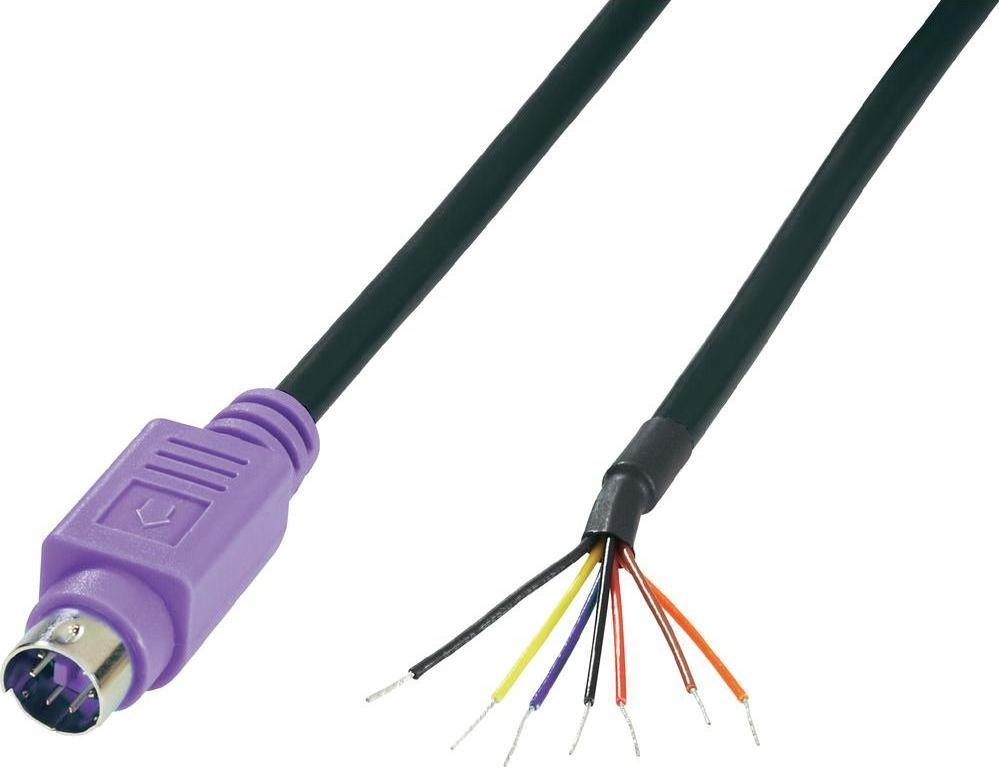
\includegraphics[width=1\textwidth]{images/ps2_male.jpg}
    \caption{PS/2 Male}
    \label{ps2_male}
  \end{minipage}
  \begin{minipage}{0.45\textwidth}
    \centering
    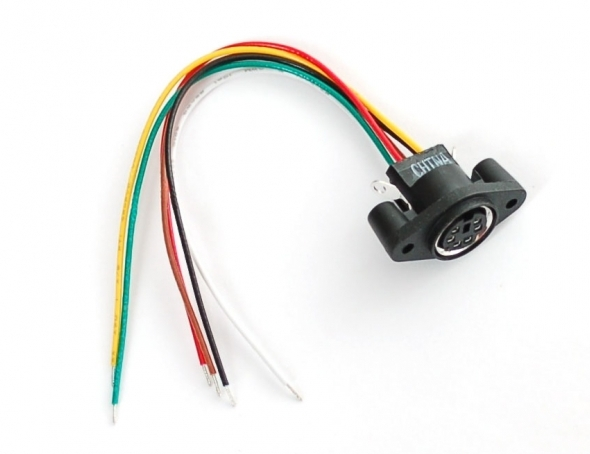
\includegraphics[width=1\textwidth]{images/ps2_female.jpg}
    \caption{PS/2 Female}
    \label{ps2_female}
  \end{minipage}
\end{figure}

\begin{figure}
  \centering
  %\includegraphics[width=0.8\textwidth]{images/hall_effect_sensor.jpg}
  \caption{Schema des Aufbaus fritzing}
  \label{fritzing}
\end{figure}

\begin{figure}
  \centering
  %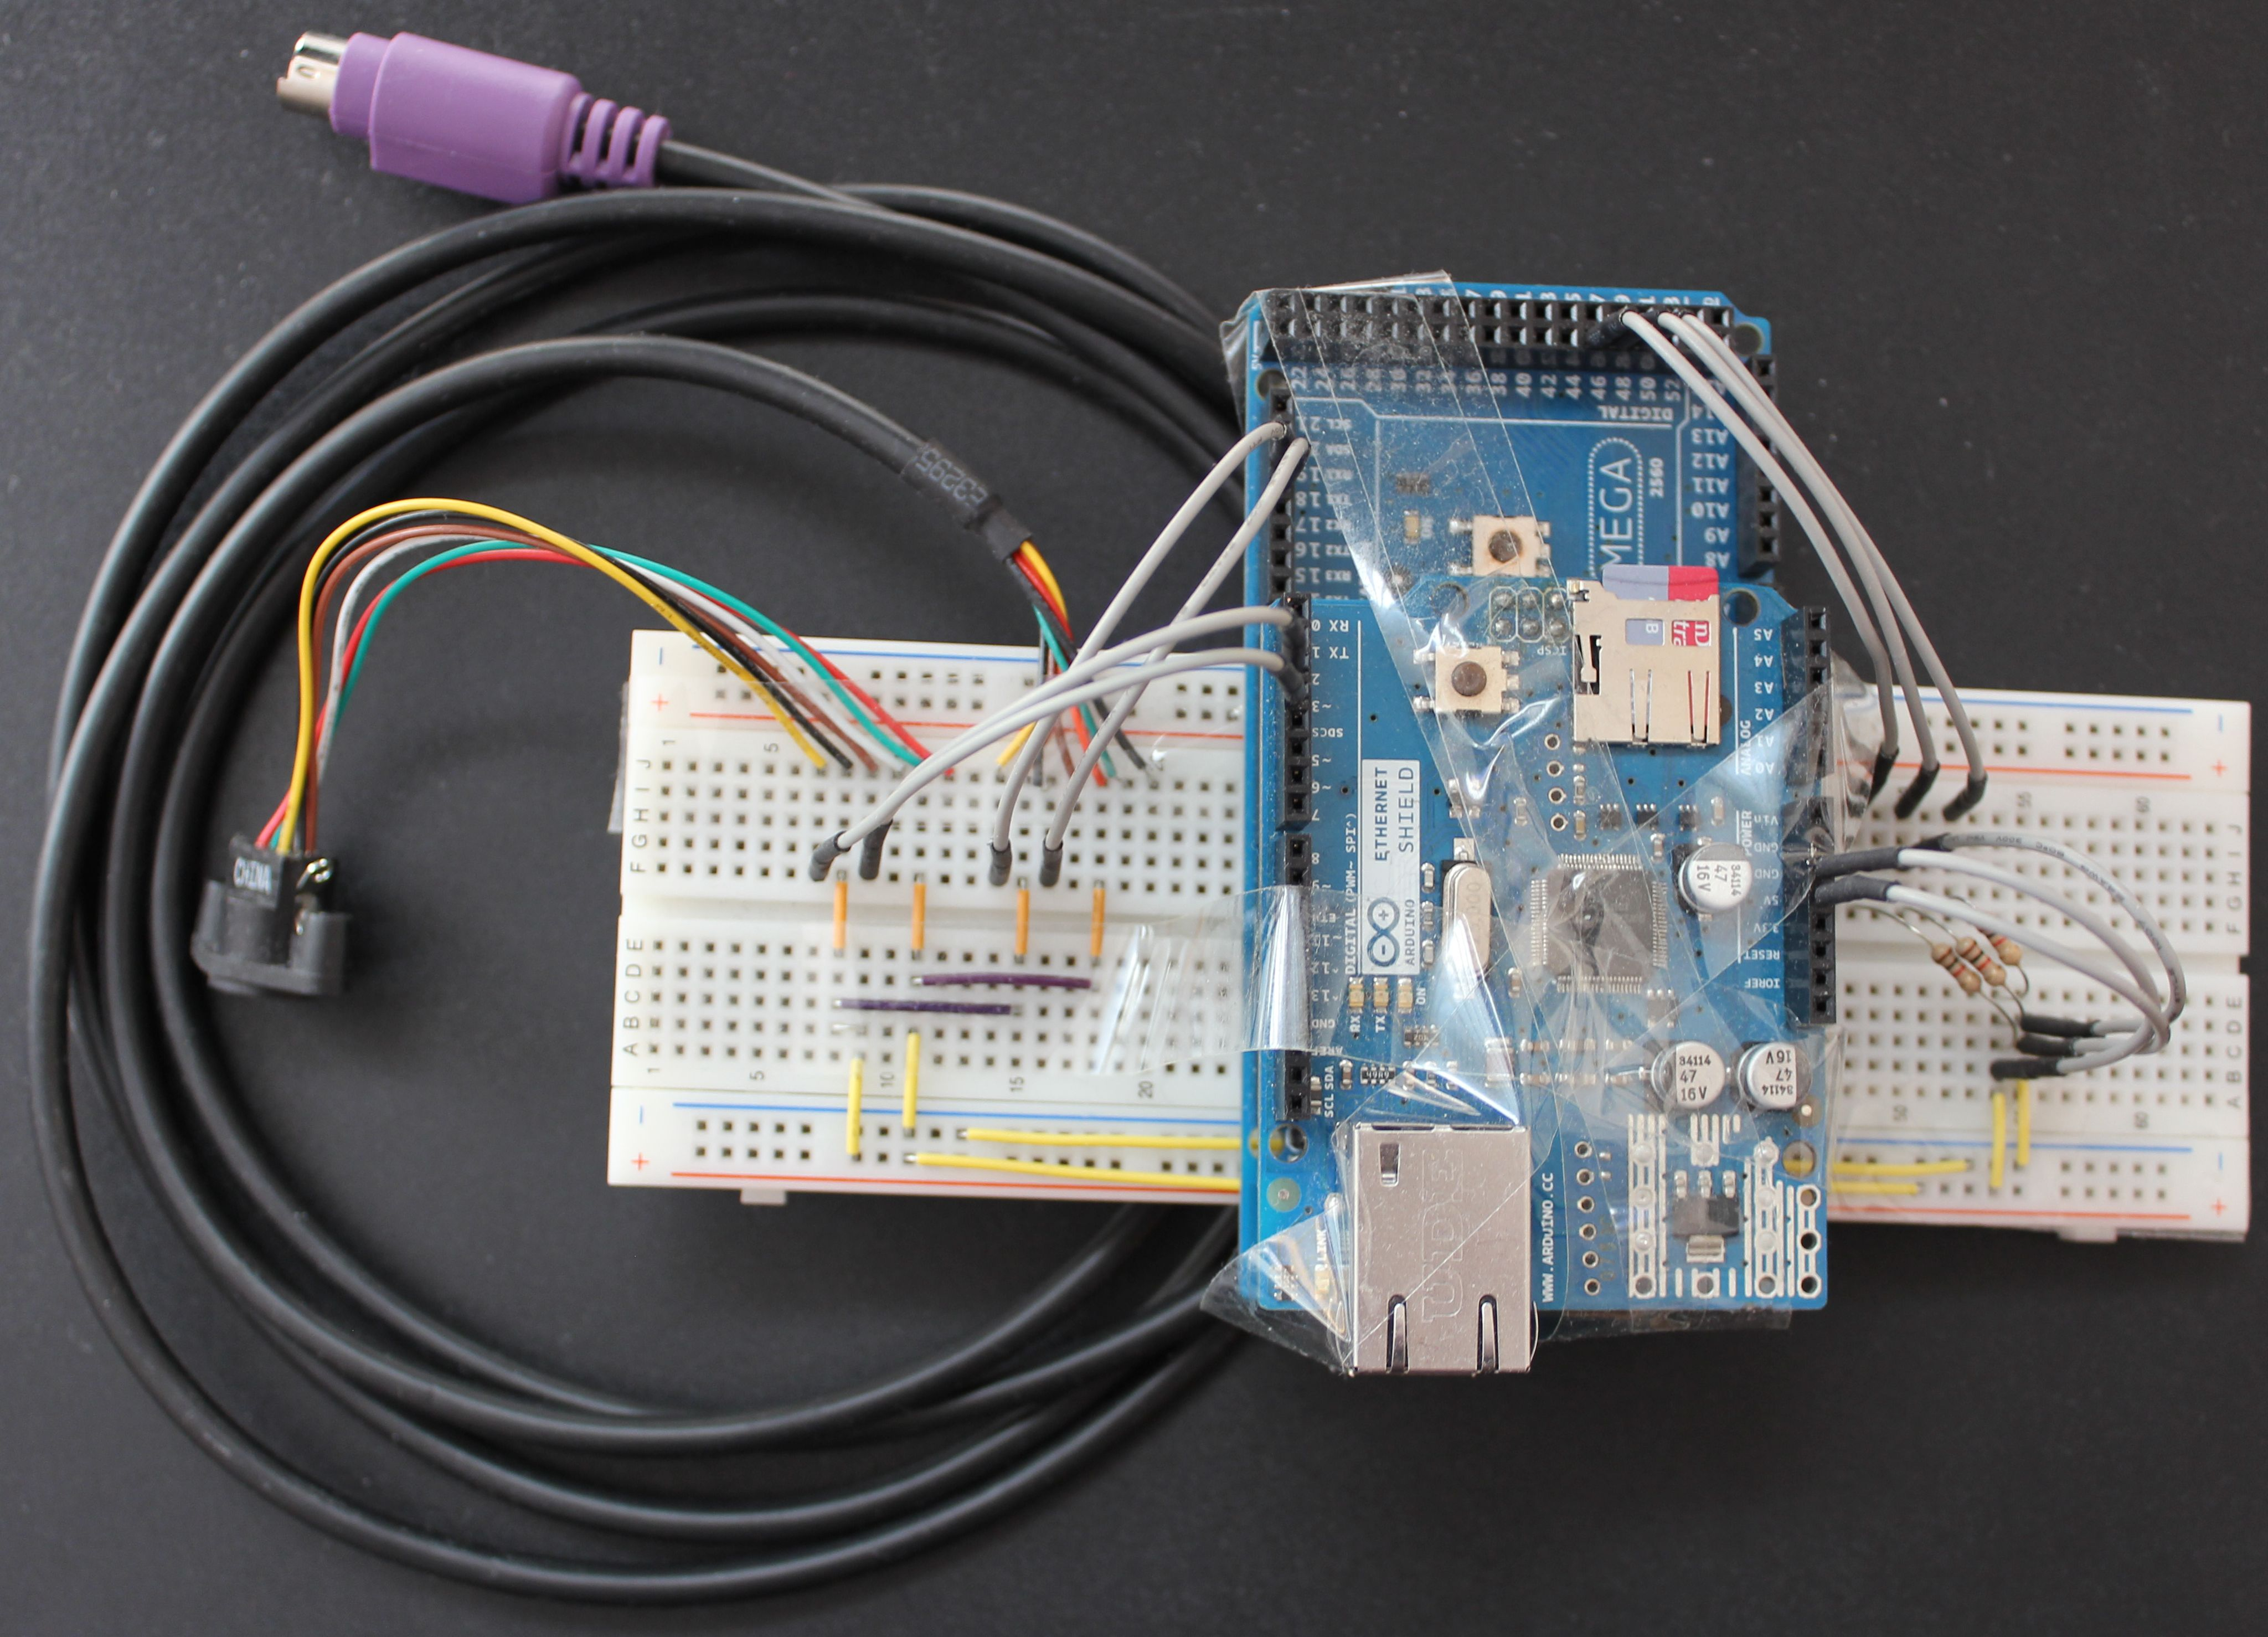
\includegraphics[width=0.8\textwidth]{images/foto1.jpg}
  \caption{Foto des Arduino Ethernet Shields und des Mega 2560 Boards}
  \label{foto1}
\end{figure}